\chapter{Développement du système}
\section{Introduction}
Le but poursuivit par ce chapitre est d'expliquer les choix qui ont influencé le développement de l'application et de chacun de ses modules externes, à savoir:

\begin{description}
  \item[ConstraintsChecker] le module qui s'occupe de vérifier la validité des programmes des étudiants;
  \item[XlsParser] le module qui s'occupe d'exporter les données des programmes de cours vers les formulaires et d'extraire les formulaires en provenance de la commission de programme;
  \item[GraphParser] le module qui s'occupe d'extraire les données en provenances des graphes que la commission de programme importe dans l'application.
\end{description}(ConstraintChecker, XlsParser et GraphParser). La structure du chapitre sera la suivante. 

La première section présentera l'architecture de l'application et de ses différents modules. On évitera ici de parler de l'architecture MVC car très peut de choix on été fait à ce niveau  (peu de libertés sont laissées par le framework au final). L'application gère et échange (avec ses modules) une grande quantité de données. Leur modélisation a un impacte critique sur les fonctionnalités de l'application (et leur implémentation). C'est pourquoi, l'accent sera mis ici sur la modélisation des classes de l'application.   

La deuxième section présentera les choix faits au niveau de l'implémentation des différentes fonctionnalités. Il sera expliqué par la même occasion comment ces fonctionnalités on été implémentées. 


\label{developpement_system}
\lhead{Chapitre 4 - Développement du système}
\section{Architecture}

\subsection{Architecture globale}

\begin{figure}
\caption{Architecture globale}
\centering
\label{fig:complete_arch}
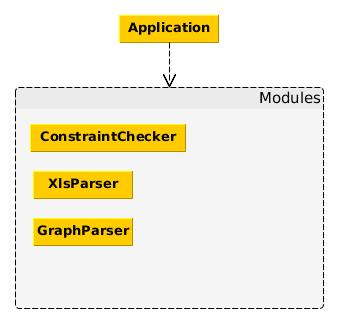
\includegraphics[width=\textwidth]{complete_arch}
\end{figure}

Ce modèle représente l'architecture de l'application et de l'ensemble de ses modules. L'objet application représente la partie \textit{Rails} de l'application. Cette partie comporte essentiellement les différents modèles, leurs vues et leurs contrôleurs (en plus de la base de données). L'application utilise trois modules développés indépendamment.
\begin{enumerate}
  \item \textbf{GraphParser} - le module s'occupant d'extraire l'information contenue dans les fichiers \textit{Graphml} générés par yEd, 
  \item \textbf{ConstraintCheker} - le module s'occupant de vérifier les contraintes des programmes d'étudiants
  \item \textbf{XlsParser} - le module occupant d'exporter les données relatives au programmes de cours vers un formulaire excel et d'extraire les informations contenues dans les formulaires excels que la commission importe via l'application. 
\end{enumerate}

Les informations manipulées par ces trois modules sont présentées en détail dans la section relative à la gestion des données du chapitre précédent \ref{data_mgmt}.

L'architecture de chacun de ces modules, en plus de celle de l'application sera expliqué dans les sous-sections qui suivent. Notez que la notation UML sera utilisée pour présenter les différents diagrammes de classe. 

Les conventions utilisées pour réaliser chacun des modèles sont les suivantes:


\begin{figure}[H]
\centering
\caption{Généralisation}
\label{fig:generalization}
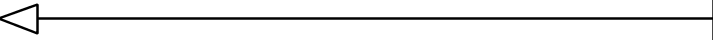
\includegraphics[width=\textwidth]{generalization}
\end{figure}

\begin{figure}[H]
\centering
\caption{Dépendance}
\label{fig:dependancy}
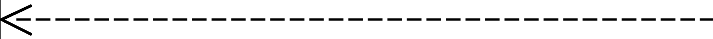
\includegraphics[width=\textwidth]{dependancy}
\end{figure}


\begin{figure}[H]
\centering
\caption{Association avec ses cardinalités}
 \label{fig:association}
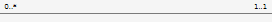
\includegraphics[width=\textwidth]{association}
\end{figure}

\begin{figure}[H]
\centering
\caption{Représentation d'une classe. En haut; les attributs, en bas; les méthodes.}
\label{fig:class_example}
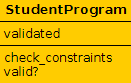
\includegraphics[scale=1]{class_example}
\end{figure}


\clearpage
\subsection{Application Rails}
\label{rails_arch}

Il y a plusieurs types d'associations en ruby on rails:
\begin{description}
  \item[Has One] - les cardinalité de cette association sont (0..1, 1..1); lorsqu'un objet A a une association \textit{has\_one} avec un objet B, B contient une référence vers l'objet A; 
  \item[Has Many] - les cardinalité de cette association sont (0..*, 1..*); lorsqu'un objet A a une association \textit{has\_many} avec un objet B, B contient une référence vers l'objet A;
  \item[Has And Belongs To Many] - les cardinalité de cette association sont (0..*, 0..*). Lorsqu'un objet a unne association \textit{has\_and\_belongs\_to\_many}, aucune référence n'est stockée dans les objets; à la place, une table intermédiaire est créée contenant l'id des deux objets.  
\end{description}

\label{arch}
\begin{figure}
\centering
\caption{Architecture de l'application}
\label{fig:app_arch}
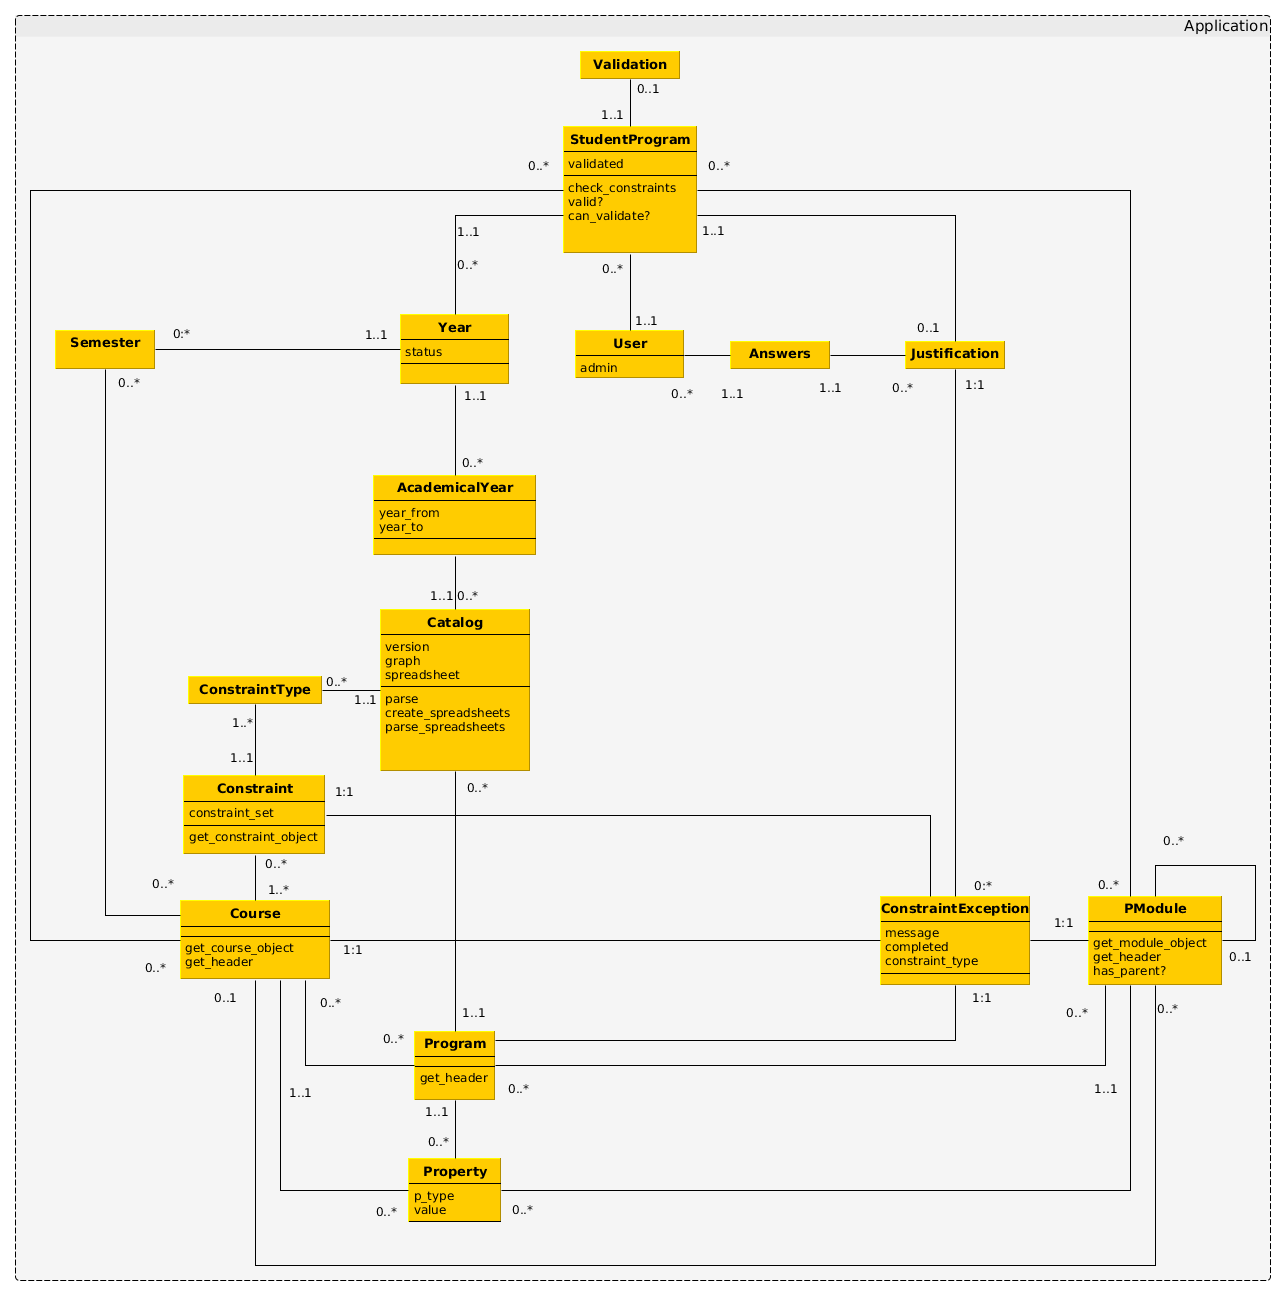
\includegraphics[width=\textwidth]{app_arch}
\end{figure}

\subsubsection{User} 

Cette classe représente les utilisateurs.  L'attribut \textbf{admin} sert à différencier les deux acteurs de l'application, à savoir la \textit{Commission de programme} et les étudiants. La section \ref{user_mgmt}
 explique en détail comment sont gérés les accès de ces deux types d'utilisateurs.

\subsubsection{Property}

Un objet \textit{Property} est composé d'un type et d'une valeur. Chacun des objets \textit{Program}, \textit{PModule} et \textit{Course} peu en avoir zéro ou plusieurs. Par exemple, pour représenter le sigle d'un cours, une propriété de type \textit{SIGLE} et de valeur \textit{SINF1101} sera ajoutée au cours correspondant. Il a été choisi d'opter pour cette solution, plutôt que d'ajouter des champs arbitraire (Sigle, crédits, ...) à chacun des objets car on ne sait pas à l'avance quelles seront leur propriété. En effet, elle sont déterminées par les informations mises dans le fichier excel qui est importé régulièrement dans l'application. 

\subsubsection{PModule}

C'est un ensemble de cours. Un \textit{PModule} peut avoir plusieurs \textit{PModule}. Ce comportement est justifié par le fait qu'un module de cours peut comporté un sous module qui comporte une série de cours obligatoires (L'option réseau et l'ensemble de ses cours obligatoires par exemple).

\subsubsection{Program}

Il représente un programme de cours. (Le programme de master par exemple) C'est un ensemble de cours et de modules divers. On peut créer des programmes via l'outil de graphes yEd, mais il est possible dans l'application de créer des Programmes \textit{à la carte} en choisissant les modules et cours qui le compose. C'est pourquoi il y a une relation \textit{many to many} entre \textit{PModule} et \textit{Program} et une autre entre \textit{Program} et \textit{Course}. En effet, chaque Programme peut avoir un ou plusieurs cours, et chaque cours peut appartenir à un ou plusieurs programmes (Le même comportement est observé pour les modules). Il n'est donc pas possible de représenter cette relation avec une relation \textit{has many} classique, qui implique d'avoir une références vers l'un des deux objets dans contenue l'autre. \cite{active_record}. 

\subsubsection{Catalog} 

Un catalogue est composé de plusieurs \textit{Program}, \textit{PModule} et \textit{Course}. Il contient aussi les informations à propos du fichier de graphe et du formulaire excel (nom, date, type). 

L'attribut \textit{version} est un entier qui représente la version du catalogue de cours. Il peut prendre trois valeurs différentes:

\begin{description}
  \item[0] version \textit{future};
  \item[1] version \textit{principale};
  \item[2] version \textit{ancienne}.
\end{description}

Les trois méthodes principales de cette classes sont:

\begin{description}
  \item[parse] qui appelle le module \textit{GraphParser}
  \item[parse\_spreadsheet] qui extrait les informations du formulaire excel (et upload la nouvelle version du formulaire sur le cloud).
  \item[create\_spreadsheet] qui crée le formulaire excel (et l'upload sur le cloud).
\end{description}

Les détails d'implémentation de ces méthodes seront expliquées dans la section relative au module avec lequel elles interagissent. 

\subsubsection{StudentProgram}

C'est le programme que se crée l'étudiant lorsqu'il utilise l'application. Un \textit{StudentProgram} est une instanciation d'un des \textit{Program} disponible dans le \textit{Catalog} utilisé (d'où la relation \textit{many to many}). De plus, un étudiant doit choisir les modules qu'il va suivre. Ce comportement est expliqué par la relation \textit{many to many} entre les deux modèles. Pour configurer son programme année par année, l'étudiant va se créer une année (\textit{Year})

La méthode \textit{can\_validate?} vérifie que certaines conditions sont remplies pour pouvoir envoyer un programme d'étudiant à la validation (Se référer à la section \ref{validation_request} pour plus de détail sur cette fonctionnalité).

La méthode \textit{check\_constraint} gère l’interaction avec le module \textit{ConstraintsChecker}. 

\subsubsection{Year}

Une année est composé de deux semestres. Un semestre est représenté par l'objet \textit{Semester}. L'attribut \textit{status} représente le fait qu'un programme d'étudiant aie été validé ou non par la commission. Le choix de chacun des cours du semestre est représenté par une association \textit{has\_and\_belongs\_to\_many} qui existe entre les deux objets.

Pour représenter le premier et le second semestre, un modèle \textit{FirstSemester} et un modèle \textit{SecondSemester} ont été créés, tout deux étendant le modèle \textit{Semester} en utilisant la \textit{Single Table Inheritance} de \textit{Rails} \cite{STI}. Notez que la relation entre ces deux types de \textit{Semester} et leur \textit{StudentProgram} est une \textit{has one} (la cardinalité est donc (1, 1) ici)

La choix d'utiliser la \textit{single table inheritance} est justifié par plusieurs raisons:
\begin{itemize}
  \item un objet \textit{year} étant composé de deux semestres, c'est plus clair d'utiliser deux associations \textit{has\_one} que d'utiliser une association \textit{has\_many} et de restreindre leur nombre par année en utilisant une validation; \textit{hardcodée}
  \item l'implémentation des formulaire de création d'année est plus aisée; on sait explicitement quel objet va représenter quel semestre;
  \item on laisse à rails le travail de devoir gérer le type de l'objet \textit{Semester} et comment devoir accéder à chacun de ceux-ci. Si l'on décide de changer le nombre de semestres par année, il suffit de créer un nouveau modèle qui étend \textit{Semester} et de rajouter la relation. Avec une solution conventionnelle, on devrait écrire du code pour représenter, créer et récupérer ce nouvel objet \textit{Semester} dans l'objet \textit{Year}. 
\end{itemize}


\subsubsection{Header}

Chacun des modèles \textit{Course}, \textit{Pmodule} et \textit{Program} contient une méthode get\_header qui renvoie une suggestion de propriétés utilisées à titre indicatif avec le module \textit{XlsParser} (voir \ref{xls_parser}) pour créer les formulaires excel. Nous avons le header suivant : \{"SIGLE", "CREDITS", "SEMESTRE", "OBLIGATOIRE"\} pour le modèle \textit{Course} par exemple.

\subsubsection{Méthodes get\_objet}
Ces méthode s'occupe de traduire les données concernant les contraintes des différents cours et modules en objet ruby. Ces objets sont par après manipulés par le module \textit{ConstraintsChecker}. 
\subsubsection{Constraints}
Cette classe représente les dépendances entre les cours. Le type de la dépendance est représenté par l'objet \textit{ConstraintType}. L'attribut \textit{set\_type} quant à lui représente le type de l'ensemble de contraintes. Comme expliqué dans la section \ref{contraintes}, une dépendance peut être une relation binaire entre un cours et sa dépendance. Elle peut être aussi une relation n-aire entre plusieurs cours et leurs dépendances.

Il existe deux association (bien qu'elles ne soient représentées que par une seule, par soucis de clarté, sur le diagramme de classes \ref{fig:app_arch}) qui relient les objets \textit{constraints} aux objets \textit{courses}. La classe \textit{Constraint} ne représentent que les contraintes de type dépendance, comme expliqué dans la section \ref{contraintes}. Ce type de contrainte ayant un cours source et un cours destination, il donc est nécessaire d'avoir deux relations.  La relation entre la destination et la contrainte est représentée par une association \textit{has\_many} entre le cours et la contrainte. La relation entre la source et la contrainte, quant à elle, est représentée par une association \textit{has\_and\_belongs\_to\_many}. 

Ce comportement est justifié par le fait que l'on accède aux contraintes depuis le cours \textit{destination}. C'est à dire que l'on va chercher les dépendances d'un cours, et non chercher la relation inverse, à savoir quels sont les cours pour lequel un cours joue le rôle de dépendance.

\subsubsection{AcademicYear}
Cette classe représente une année académique, c'est à dire composé de deux années. Elle est utilisée dans deux situations:
\begin{enumerate}
  \item identifier les objets \textit{Year} et \textit{Catalogue};
  \item gérer, du coté du module \textit{ConstraintsChecker} les dépendances de cours (on peut ainsi savoir quand à été suivit un cours). 
\end{enumerate}

\subsection{Architecture du vérificateur de contraintes}
\label{constraint_checker}
\begin{figure}[H]
\centering
\caption{Vérificateur de contraintes}
\label{fig:constraint_checker_arch}
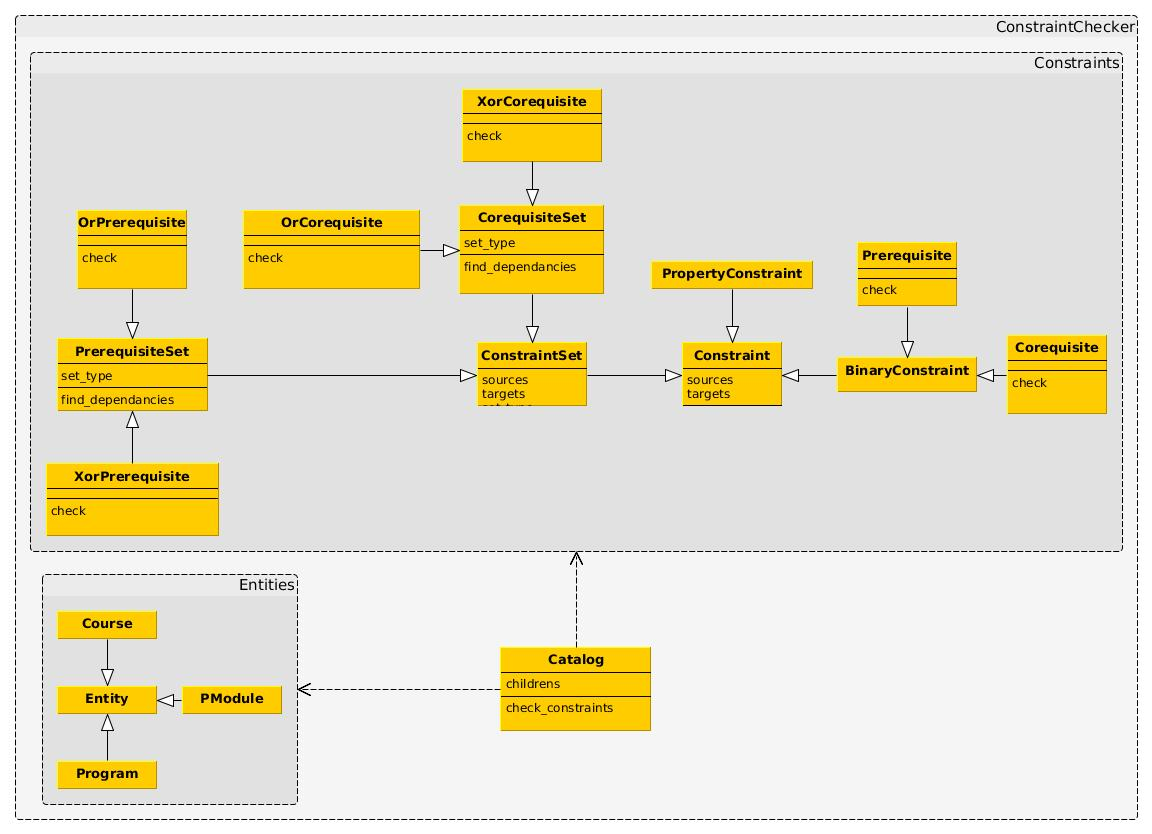
\includegraphics[width=\textwidth]{constraint_checker_arch}
\end{figure}

L'architecture de ce module est composé en deux parties;
\begin{enumerate}
  \item Les différents types de contraintes (Contraintes binaires, ensemble de contraintes ...)
  \item Les différents types d'entités (Cours, modules, ...)
\end{enumerate}

Le lien avec l'application se situe au niveau de la classe \textit{Catalog}. En effet, chacune des différentes entrées des tables concernées (courses, p\_modules, constraints) sont traduites en un objet entité.

L'idée ici est d'utiliser au plus l'héritage pour éviter d'avoir des duplications de code dans les classes. Par exemple, un objet \textit{Course} peut avoir beaucoup de contraintes mais chacune d’entre elles peut être de n'importe quel type. Cet objet n'a pas besoin de savoir le type de ses contraintes. Tout ce qu'il sait, c'est qu'il doit appeler leur méthode \textit{check} pour tester si les contraintes sont vérifiées. 


\subsection{Parser de graphes}

\begin{figure}[H]
\centering
\caption{Architecture du parser de graphe}
\label{fig:graph_parser_arch}
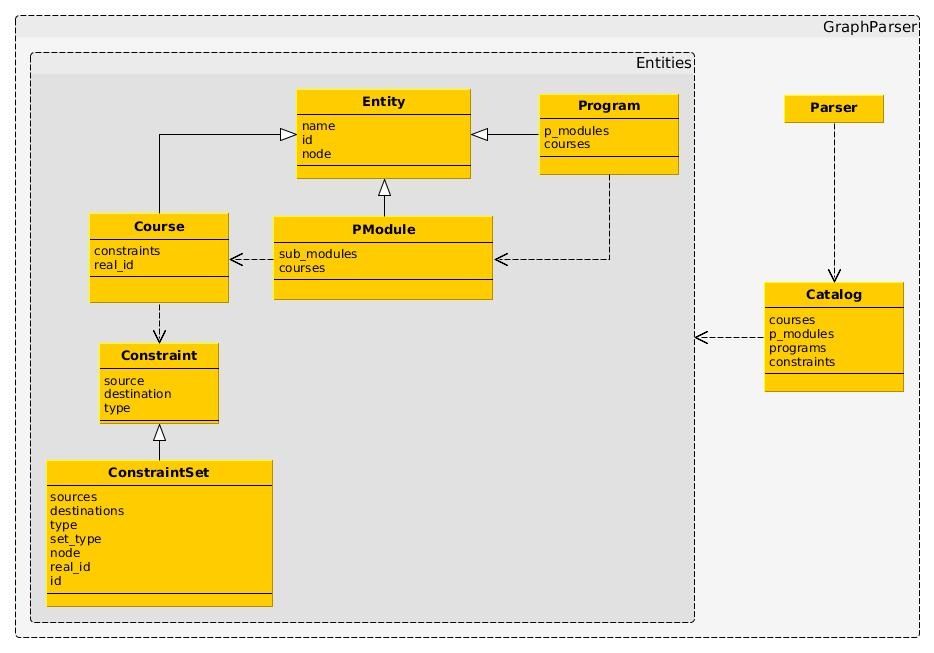
\includegraphics[width=\textwidth]{graph_parser_arch}
\end{figure}

Tout comme dans le vérificateur de contraintes \ref{constraint_checker}, le parser travail avec des objets \textit{entités} à la différence que c'est lui qui les fournit à l'application (et pas l'inverse)

De nouveau, l'héritage tient une page prépondérante ici, pour diminuer le couplage, augmenter la cohésion  et éviter autant que possible la duplication de code \cite{cohesion_couplage}. 

\subsection{Parser de fichiers excel}
\label{xls_parser}
\begin{figure}[H]
\centering
\caption{Architecture du parser de fichiers excel}
\label{xls_parser_arch}
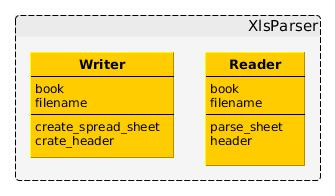
\includegraphics[scale=1]{xls_parser_arch}
\end{figure}

Ce module est relativement simple; il est composé de deux classe, un \textit{Writer} qui prend en input un tableau de donnée et un \textit{Reader} dont l'output est aussi un tableau de donnée.


\clearpage
%*************************************************************************************************************************************
\section{Implémentation}
\subsection{Hébergement de l'application}
L'application est hébergée sur \textit{Heroku}. Cela impose cependant quelques restrictions;
\begin{enumerate}
  \item On obligé d'utiliser postgresql comme système de base de données.
  \item Le répertoire de l'application est en lecture seule. On ne peut donc pas stocker le fichier de graphe et le formulaire excel dedans. Il est donc nécessaire d'utiliser un service de \textit{cloud storage} externe à l'application. Amazon S3 à été utilisé pour palier à ce problème. Pour rendre le téléchargement des fichiers vers ce service plus aisé, la gem \textit{Paperclip} a été utilisé. Les détails de configuration de ces différents services sont expliqués en annexes. 
\end{enumerate}
\subsection{Gestion des utilisateurs}
\label{user_mgmt}
Les utilisateur sont gérés à l'aide de deux gems. 

Devise est utilisé pour tout ce qui concerne la gestion des comptes (Création, modification, suppression), la gestion des sessions (Login/logout) et surtout la création de la table users et des différents attributs requis.

CanCan est utilité pour tout ce qui concerne les permissions des utilisateurs, à savoir à quel modèles un utilisateur à accès, et quels actions il peut effectuer sur ces modèles (Read, Create, Destroy, ...) 

Pour gérer les deux types d'utilisateur (Commission INFO et Étudiants, trois choix s'offrent à nous;
\begin{enumerate}
  \item générer avec devise deux tables séparées
  \item utiliser la Single Table Inheritance \cite{STI}. On crée un modèle user, puis on crée deux modèles spécifiques (student et admin) qui hérite de ce premier modèle
  \item générer un seul modèle user et y ajouter un attribut \textit{admin} pour identifier le rôle de l'utilisateur
\end{enumerate}

La troisième solution a été choisie. Elle permet d'éviter la redondance induite par la première solution et est plus simple à implémenter et à maintenir que la deuxième solution. En effet nos deux types d'utilisateur ne diffèrent que par leur rôle. 


La table générée par devise est la suivante;

\begin{lstlisting}
  create_table "users", force: true do |t|
    t.string   "email",                  default: "",    null: false
    t.string   "encrypted_password",     default: "",    null: false
    t.string   "reset_password_token"
    t.datetime "reset_password_sent_at"
    t.datetime "remember_created_at"
    t.integer  "sign_in_count",          default: 0,     null: false
    t.datetime "current_sign_in_at"
    t.datetime "last_sign_in_at"
    t.string   "current_sign_in_ip"
    t.string   "last_sign_in_ip"
    t.datetime "created_at"
    t.datetime "updated_at"
    t.boolean  "admin",                  default: false
  end
\end{lstlisting}

Pour vérifier si un utilisateur est connecté dans les vues, il suffit d'appeler le helper suivant

\begin{lstlisting}
user_signed_in?
\end{lstlisting}

Cela nous permet par exemple de cacher à l'utilisateur les menus permettant accéder aux différentes vues s'il n'est pas connecter

Pour vérifier si l'utilisateur à le rôle admin, il suffit de vérifier l'attribut dans la vue

\begin{lstlisting}
current_user.admin?
\end{lstlisting}

current\_user représentant l'utilisateur qui est connecté pour le moment.


Cependant, cela n'est pas suffisant. En effet, cela n'empêche pas l'utilisateur d'accéder aux différentes vues en entrant l'url dans la barre de navigation. C'est pourquoi il est nécessaire de dire à chaque contrôleur qu'il faut vérifier qu'un utilisateur est connecté avant d'afficher les vues. C'est fort heureusement très simple à faire avec Devise. Il suffit d'ajouter la ligne 
\begin{lstlisting}
before_action :authenticate_user!
\end{lstlisting}

dans chaque contrôleur où il est nécessaire que l'utilisateur soit connecté pour accéder aux vues. 

\textit{CanCan} intervient pour gérer les accès autorisés aux deux rôles de notre application (Utilisateur normal et admin). Il suffit simplement de créer un modèle \textit{Ability} dans lequel on décrit ce à quoi chaque rôle à accès. C'est de nouveau très simple;

\begin{lstlisting}
    if user.admin?
        can :manage, :all
    else
        can :manage, [StudentProgram, Year, Semester]
        can :create, Validation
    end
\end{lstlisting}

Il suffit de définir, en fonction du rôle de l'utilisateur, les modèles auxquels il a accès et ce qu'il peut faire. L'utilisateur \textit{normal} par exemple, n'a accès qu'aux modèles \textit{StudentProgram, Year, Semester}. S'il tente d'accéder aux vues des modèles auxquels il n'a pas accès, il sera redirigé vers la page d’accueil. 

Notez qu'il est possible de générer les vues qui permettent à l'utilisateur de s'enregistrer, de se connecter et de gérer les informations relatives à son compte utilisateur. Ces vues ont cependant été modifiées pour que leur style s'adapte à celui de l'application. 

Enfin, il n'est pas possible, pour des questions de sécurité évidentes, de se créer un compte \textit{admin} via les formulaires d'enregistrement disponibles dans l'application. Il faut tout d'abord se créer un compte utilisateur dans l'application, et ensuite modifier l'attribut \textit{admin} directement dans la console.  

\subsection{Importation du graphe}
\subsubsection{Introduction}
\label{graph_format_justification}
Une fois le graphe créé à l'aide de yEd, plusieurs choix s'offrent à nous pour exporter nos données. Les formats (non binaires) dans lesquels nous pouvons exporter les informations contenues dans notre graphe sont les suivantes. 
\begin{enumerate}
\item GraphML, un format de fichier basé sur XML pour les graphes
\item XGML, une alternative au format GraphML, mise en place par yWorks, la société qui développe le logiciel yEd
\item TGF (Trivial Graph Format) un format de fichier texte relativement simple pour décrire des graphiques
\end{enumerate}

TGF est de la forme

\begin{lstlisting}
1 SINF1101
2 FSAB1401
3 SINF1103
4 SINF1102
5 SINF1140
6 INGI1123
7 INGI1101
8 FSAB1402
9 NS //(Option network & security du programme Master)
\end{lstlisting}

et contient trop peu d'informations sur le graphe, comme les appartenances des cours aux différents modules et programmes. C'est pourquoi une solution basée sur XML a été choisie.

Voici ce à quoi ressemble les informations d'un fichier GraphML pour un noeud de type COURS.

\begin{lstlisting}
 <node id="n1::n3" yfiles.foldertype="group">
  <data key="d5"/>
    <data key="d6">
    (...)
  <node id="n1::n3::n2">
      <data key="d5"/>
      <data key="d6">
        <y:ShapeNode>
          <y:Geometry height="30.0" width="68.0" x="1136.0" y="1541.453125"/>
          <y:Fill color="#FFCC00" transparent="false"/>
          <y:BorderStyle color="#000000" type="line" width="1.0"/>
          <y:NodeLabel alignment="center" autoSizePolicy="content" fontFamily="Dialog" fontSize="12" fontStyle="plain" hasBackgroundColor="false" hasLineColor="false" height="17.96875" modelName="internal" modelPosition="c" textColor="#000000" visible="true" width="61.57421875" x="3.212890625" y="6.015625">SINF2335</y:NodeLabel>
          <y:Shape type="rectangle"/>
        </y:ShapeNode>
     </data>
  </node>
  (...)
</node>
\end{lstlisting}

En comparaison, la version \textit{XGML} du même nœud.
\begin{lstlisting}
<section name="node">
  <attribute key="id" type="int">69</attribute>
  <attribute key="label" type="String">SINF2335</attribute>
  <section name="graphics">
    <attribute key="x" type="double">1170.0</attribute>
    <attribute key="y" type="double">1556.453125</attribute>
    <attribute key="w" type="double">68.0</attribute>
    <attribute key="h" type="double">30.0</attribute>
    <attribute key="type" type="String">rectangle</attribute>
    <attribute key="fill" type="String">#FFCC00</attribute>
    <attribute key="outline" type="String">#000000</attribute>
  </section>
  <section name="LabelGraphics">
    <attribute key="text" type="String">SINF2335</attribute>
    <attribute key="fontSize" type="int">12</attribute>
    <attribute key="fontName" type="String">Dialog</attribute>
    <attribute key="anchor" type="String">c</attribute>
  </section>
  <attribute key="gid" type="int">61</attribute>
</section>
\end{lstlisting}

La principale différence entre le format XGML et GraphML se situe au niveau de la structure des informations. XGML structure toute les données de façon linéaire, en ne respectant pas la hiérarchie des différents nœuds et boites.

\begin{figure}
\centering
\caption{Exemple de graphe hiérarchique} 
\label{fig:hierarchical_graph_example}
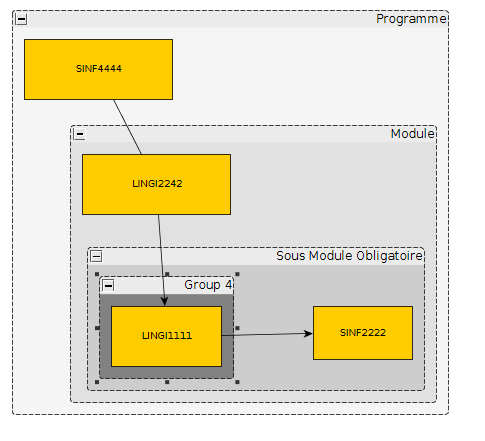
\includegraphics[width=\textwidth]{hierarchical_graph_example}
\end{figure}

Pour le graph \ref{fig:hierarchical_graph_example} par exemple, la structure d'un fichier XGML sera de la sorte:
\begin{lstlisting}
Node Programme
Node SINF4444
Node MODULE
Node LINGI2242
Node SOUS MODULE OBLIGATOIRE
(...)
\end{lstlisting}

Lorsque l'on parsera le fichier, on devra:
\begin{itemize}
  \item Parcourir le fichier, extraire les informations (nom, parent) de chaque cours, module et programme;
  \item Parcourir la liste des cours, modules et programmes pour ajouter les références vers leur parent et leurs enfants.
\end{itemize} 

Avec GraphML par contre, la structure  du fichier sera la suivante;

\begin{lstlisting}
Node Programme
Childs : [
  Node SINF4444
  Node MODULE
  Childs : [
    Node LINGI2242
    Node SOUS MODULE OBLIGATOIRE
    Childs : [
    ]
  ]
]
(...)
\end{lstlisting}

Lorsqu'on parsera le fichier; on devra simplement extraire les informations comme précédemment. On saura par contre au moment ou l'on parse un objet à quel parent il appartient.  Il n'est donc pas nécessaire de retraiter tout les éléments pour compléter les informations à propos de leur parent et de leurs enfants. Ceci est la principale raison pourquoi \textit{Graphml} est le format supporté par l'application.


\subsubsection{Parsing}
\label{graph_parsing}
Le but de ce module est de fournir une abstraction supplémentaire à la gem \textit{Nokogiri}\footnote{Librairie ruby permettant de parser des fichiers XML} pour extraire les informations contenues dans le fichier \textit{GraphML} de yEd. Les informations contenue dans le graphe généré avec \textit{yEd} sont les suivantes:
\begin{itemize}
\item Les Programmes de cours (Bachelier, Masters)
\item Les Modules et leur nom
\item Les Sous-modules et leur nom
\item Les cours et leur sigle
\item Les contraintes hiérarchiques (Qui contient quoi)
\item Les dépendances entre les cours (Corequis et Prérequis)
\end{itemize}

Ce module est appelé par le modèle \textit{Catalogue} de l'application à sa création. Le fichier graphe est d'abord envoyé sur le  \textit{cloud amazon}, puis parsé par le module \textit{GraphParser}. Une fois le parsing terminé, les différents objets (Cours, Modules et Programmes) sont récupérés par le modèle \textit{Catalogue}, puis traités par chacun des modèles concernés, avant d'être enregistrés en base de données. 

Tout ces éléments sont représentés par des nœuds dans le fichier GraphML. Seul les dépendances entre les cours sont représentées par des arrêtes dans le graphes, nommées \textit{Edge} dans le fichier. Les nœuds sont stockés en premier dans le fichier de graphe, suivit par toute les arrêtes. 

Le module ajoutes deux fonctionnalités à \textit{Nokogiri}.
\begin{enumerate}
  \item Il parse un fichier GraphML et extrait les métadonnées de ses nœuds (type, enfants, parent) et arrêtes (source, destination, type de contrainte, type de l'ensemble de contrainte). 
  \item Il renvoie des objets cours, modules et programmes ainsi que leur différentes dépendances.  
\end{enumerate}

 Comme expliqué dans l'introduction de cette section, chaque élément peut avoir un enfant, est identifié par un tag, peut avoir des attributs et contient de l'information. 

 la structure plus détaillée d'un nœud est la suivante:

\begin{lstlisting}
<node id="parentID::nodeID" [GROUP]>
  <(...)>
  </(...)
  <NodeLabel>
    NAME
  </(...)
  <(...)>
  </(...)>
</node>
<graph id="parentID">
  <node id (...)>
  <node id (...)>
</graph>
\end{lstlisting}

Il y a donc quatre informations à extraire;
\begin{enumerate}
  \item l'identifiant du nœud parent (parentID);
  \item l'identifiant du nœud (nodeID);
  \item son nom (NAME);
  \item est-ce un groupe? (GROUP)
\end{enumerate}

La structure de graphe imposée à la commission est la suivante; 

\begin{itemize}
\item les modules et programmes sont représentés par des nœuds \textit{Group};
\item les cours sont représentés par des simple nœuds;
\item les dépendances par des arrêtes.
\end{itemize}

Notez que chaque cour et module \textbf{DOIT} se trouver dans un programme. En effet, \textit{nœuds groupes} sans parents sont interprétés comme programmes. Cela nous permet de distinguer les modules des programmes, sans devoir ajouter une convention de couleur sur les boites pour les différencier.  

L'algorithme de parsing est donc relativement simple.

On a;
\begin{itemize}
  \item une méthode qui parse les arrêtes; 
  \item une méthode qui parse les nœuds;
  \item une méthode qui aprse les programmes et ses enfants;
  \item une méthode qui parse les modules et ses enfants;
  \item une méthode qui parse les cours.
\end{itemize}

On crée au préalable un \textbf{objet} catalogue. Chacune des méthodes listées précédemment renvoie un \textbf{objet} Cours, Module, Programme, Contrainte. Ces objets sont ajoutés au catalogue en respectant leur hiérarchie. Un cours aura donc comme parent un module ou un programme. 


\begin{lstlisting}
FOREACH element in graph do
- IF node -> 
  parse node
  - IF program -> 
    parse program (extract informations and add to catalog)
    (1) parse childs
      - IF module
        -> parse module (extract informations and add to parent)
        -> parse childs (go_to (1))
      - IF course
        -> parse course (extract informations and add to parent)


- IF edge -> 
  parse edge
    retrieve sources
    retrieve destinatinations
    retrieve constraint type
    FOREACH course in destinations do
      add new contraint to course
\end{lstlisting}


Une fois le parsing terminé, toutes les informations contenues dans chacun des \textbf{objets} cours, modules et programmes et contraintes sont ajoutés dans la table correspondante en base de donnée. 


\subsection{Gestion des contraintes}
Les contraintes sont vérifiées au niveau du modèle \textit{StudentProgram}, le modèle qui contient les informations à propos des programmes de cours des étudiants (C'est ce modèle qui appelle le module \textit{ConstraintsChecker}. 

Le module \textit{ConstraintsChecker} est divisé en deux parties. D'un coté nous avons les contraintes. Tout les types de contraintes héritent de la super classe \textit{Contrainte} qui, en plus de constructeur ne contient qu'une seule méthode \textbf{Check}. De l'autre coté nous avons les entités qui représentent les modèles \textit{Course}, \textit{Module} et \textit{Program}

\subsubsection{Entités}
\textit{Entity} est la classe qui représente les objets traités par le module \textit{ConstraintsChecker}. Entity étends la classe OpenStruct. Openstruct est une librairie qui permet de créer des objets à la volée. Pour chaque paramètre passé à un objet \textit{OpenStruct} \cite{OpenStruct}, un attribut sera créé ainsi que les méthodes pour le modifier et y accéder. On évite ainsi de devoir modifier la classe \textit{Entity} et ses enfants {Course, PModule} lorsque l'on veut rajouter une contrainte ou une nouvelle propriété par exemple.

Nos différents objets sont stockés sous forme d'arbre. La racine est l'objet catalogue, et les enfants sont les différents objets \textit{Course} et \textit{PModule}, tous étendant le super-type \textit{Entity}.

Un objet \textit{entity} contient essentiellement;

\begin{itemize}
  \item un attribut \textbf{constraints} qui contienne les différentes contraintes de l'objet;
  \item un attribut \textbf{childrens} qui contient les références vers ses enfant dans l'arbre;
  \item un attribut \textbf{parent} qui contient la référence vers son parent dans l'arbre;
  \item une méthode \textbf{find\_children(children\_id, children\_type)} qui permet d'effectuer une recherche sur ses enfants. Le paramètre \textit{children\_type} permets de spécifier le type d'enfant que nous recherchons (Cours, PModule);
  \item une méthode \textbf{search(children\_id, children\_type)} qui permet d'effectuer une recherche dans tout l'arbre. Cette méthode est utilisé dans les methodes \textit{check} des différentes contraintes pour retrouver des objets \textit{Course}. (Retrouver une dépendance par exemple). L'algorithme est le suivant;
  \begin{lstlisting}
  - Retrouver la racine de l'arbre
  - Appeler find_children sur ses enfants
  \end{lstlisting}
  \item une méthode \textbf{check} qui vérifie ses contraintes et celle de ses enfants;
  \item des méthodes relatives aux différentes contraintes, comme \textit{count\_credits}, \textit{check\_max}, \textit{check\_min}, \ldots
\end{itemize}

Ces objets sont construits dans les différents modèles de l'application. L'idée, dans chacun de ces modèles (Course, PModule, Constraint) est d'avoir une méthode get\_[model\_name]object qui va créer l'objet correspondant.

Dans le cas du modèle \textit{Course}, la méthode est la suivante:


\textbf{Course}

\begin{lstlisting}
def get_course_object(start_year, end_year)
  course = ConstraintsChecker::Entities::Course.new(name: self.name, id: self.id, start_year: start_year, end_year: end_year, parent_id: self.p_module_id, credits: self.credits, mandatory: self.mandatory?)
  self.constraints.each do |c|
    course.add_constraint(c.get_constraint_object(course))
  end
  return course
end
\end{lstlisting}


Les paramètre \textit{start\_year} et \textit{end\_year} identifient l'année académique au cours de laquelle un cours a été suivie dans un programme d'étudiant. Ces informations sont utilisés lors de la vérification des dépendances. 

Dans le cas d'un prérequis  par exemple, l'algorithme va vérifier que l'année académique durant laquelle a été suivie le cours est strictement antérieure à l'année académique du cours pour le quel il est un prérequis. Ce mécanisme gère aussi bien les années réussies que les années ratées. En effet, dans le cas d'une année raté, la commission aura au préalable sélectionner les cours qui on été réussis. Les cours ratés (qui ne sont pas sélectionnés) seront retiré de l'année en question. Il ne seront donc pas présent dans \textbf{objet} catalogue lors de la vérification des contraintes. 

Comme expliqué plus haut, on peut passer au constructeur de \textit{Course} tout ce que l'on veut, grâce à OpenStruct \cite{OpenStruct}.

Rien ne nous oblige à passer par le modèle \textit{Constraint} pour ajouter les contraintes. Comme expliqué dans la section \ref{rails_arch} (présentant l'architecture de l'application) , seul les dépendances sont représentés par l'objet \textit{Constraint} en base de données. En effet la plupart des données relatives à ces contraintes sont, en plus d'être présentes en base de données, assez volatiles, car elles peuvent être modifiées régulièrement via l'import de fichiers excels. Nous évitons ainsi de surcharger notre architecture avec des objets dont l'utilité est plus que relative. Pour revenir à ce type de contraintes, il est préférable de les ajouter dans la méthode \textit{get\_[model\_name]object} (la méthode du modèle qui crée l'objet \textit{Entity}.

\textbf{PModule}

\begin{lstlisting}
def get_p_module_object(mandatory)
  p_module = ConstraintsChecker::Entities::PModule.new(id: self.id, name: self.name)
  p_module.add_constraint(ConstraintsChecker::Constraints::Min.new(p_module, self.min))-
  p_module.add_constraint(ConstraintsChecker::Constraints::Max.new(p_module, self.max))
  self.sub_modules.each do |m|
    p_module.add_children(m.get_p_module_object(true))
  end

  if mandatory
    course_ids = []
    self.courses.each do |course|
      course_ids << course.id
    end
    p_module.add_constraint(ConstraintsChecker::Constraints::Mandatory.new(p_module, course_ids))
  end

  return p_module
end
\end{lstlisting}

Le paramètre \textit{mandatory} sert à identifier si le module est obligatoire ou non. Cela est utile pour vérifier si les cours d'un module obligatoire on bien été suivis.
Nous avons ici un exemple de contraintes (Min \& Max) qui ne sont pas ajoutées en passant par le modèle \textit{Constraint}. 


\subsubsection{Contraintes}
L'idée, pour chaque type de contraintes, est d'étendre la super-classe \textit{Constraint} en ré-implémentant la méthode \textit{check} pour qu'elle corresponde au comportement recherché. Cette méthode renvoie un \textit{hash}, spécifique à chaque type de contraintes, contenant les résultats de la vérification.

Par exemple, pour les dépendances entre les cours nous avons deux types. Les dépendances binaires, qui correspondent à un prérequis ou corequis entre deux cours, et les dépendances n-aire qui correspondent à un ensemble de prérequis ou corequis entre plusieurs cours avec une condition sur cet ensemble de contraintes. Cet ensemble peut être une disjonction (OR) de contraintes par exemple, exprimant qu'il faut choisir au moins une des dépendances, ou une disjonction exclusive (XOR), exprimant qu'il faut choisir une et une seule dépendance. 

Prenons l'exemple des dépendances binaires. Nous avons une classe \textit{BinaryConstraint} qui ne ré-implémente pas la méthode check de sa super-classe \textit{Constraint} car elle sert de super-classe pour les deux classes représentant les deux types de contraintes; \textit{Prerequisite} et \textit{Corequisite}. 

\begin{description}
  \item[Corequisite] La méthode check va appeler la méthode \textit{find\_course} du cours en question, qui va remonter jusqu'à la racine (le catalogue), et chercher si le corequis du cours est présent dans le catalogue.  S'il est présent, il va vérifier qu'il n'est pas suivit dans une année postérieure au cours pour le quel il est un corequis (conformément à la définition d'un prérequis \ref{contraintes}). Si la vérification précédente échoue, ou si le cours n'est tout simplement pas présent, le message ``corequisite\_missing :[course\_id]'' est envoyé.
  \item[Prerequisite] La méthode check se comporte comme celle de \textit{Corequisite}, à la différence que la vérification de l'année académique est plus stricte: le cours doit être suivit dans une année strictement antérieure (conformément à la définition d'un prérequis \ref{contraintes}). 
\end{description}

Dans le cas d'un ensemble n-aire de contraintes, il y a essentiellement deux points qui diffèrent;
\begin{enumerate}
  \item l'existence d'une méthode \textit{find\_dependancies} qui récupère les \textit{course\_id} manquants pour la contrainte en question en vérifiant aussi les années académiques;
  \item une vérification sur la taille de la liste, correspondant à la condition qui régit cet ensemble de contrainte. Dans le cas d'un ensemble disjonctif (OR), il faut vérifier que le nombre de \textit{course\_id} renvoyé soit strictement inférieure au nombre de dépendances du cours, pour vérifier qu'il y ai au moins une dépendance qui est choisie, conformément à la logique d'une disjonction. Dans le cas d'un ensemble disjonctif exclusif (XOR), il faut vérifier qu'il n'y aie qu'une et une seule dépendance choisie, conformément à la logique d'une disjonction exclusive.
\end{enumerate}

Pour vérifier ces contraintes, l'objet \textit{Catalog} appelle sur chacune des contraintes de ses enfants et de leur enfants leur méthode \textit{check} et récupère les messages qu'elles renvoient. Ces messages sont traités par le modèle \textit{StudentProgram} et affichés sur les vues correspondantes.

À ce jour, la liste des messages renvoyés par les méthodes \textit{check} des différents types de contraintes est la suivante:

\begin{description}
\item[or\_corequisites\_missing] Ce message concerne la contrainte n-aire \textit{OR-Corequisite}. Il contient la liste des ids des cours concernés par la contrainte si elle n'est pas vérifiée;
\item[xor\_corequisites\_missing] Ce message concerne la contrainte n-aire \textit{XOR-Corequisite}. Il contient la liste des ids des cours concernés par la contrainte si elle n'est pas vérifiée;
\item[or\_prerequisites\_missing] Ce message concerne la contrainte n-aire \textit{OR-Prerequisite}. Il contient la liste des ids des cours concernés par la contrainte si elle n'est pas vérifiée;
\item[xor\_prerequisites\_missing] Ce message concerne la contrainte n-aire \textit{XOR-Prerequisite}. Il contient la liste des ids des cours concernés par la contrainte si elle n'est pas vérifiée;
\item[prerequisites\_missing] Ce message concerne la contrainte binaire \textit{Prerequisite}. Il contient l'id du cours concerné par la contrainte si elle n'est pas vérifiée;
\item[corequisites\_missing] Ce message concerne la contrainte binaire \textit{Corequisite}. Il contient l'id du cours concerné par la contrainte si elle n'est pas vérifiée;
\item[to\_few\_credits] Ce message concerne la contrainte sur la propriété (Crédits) \textit{Min}. Il contient l'id de l'entité concerné par la contrainte si elle n'est pas vérifiée;
\item[to\_many\_credits] Ce message concerne la contrainte sur la propriété (Crédits) \textit{Max}. Il contient l'id de l'entité concerné par la contrainte si elle n'est pas vérifiée;
\item[courses\_missing\_in\_module] Ce message concerne la contrainte sur la propriété \textit{Mandatory} d'un objet \textit{Module}. Il contient les ids des entités manquantes d'un Module; obligatoire si la contrainte n'est pas vérifiée;  
\item[mandatory\_courses\_missing] Ce message concerne la contrainte sur la propriété \textit{Mandatory} d'un objet \textit{Course}. Il contient l'id du cours en question si la contrainte n'est pas vérifiée.
\end{description}

Pour ajouter un nouveau type de contraintes, il faut procéder comme suit;

\begin{enumerate}
  \item Si le type de la contrainte ne rentre pas dans la catégorisation des contraintes déjà existantes (BinaryConstraint, PropertyConstraint, NaryConstraint), il faut créer une nouvelle classe. Sinon, il suffit d'étendre la classe existante.
  \item Implémenter la méthode \textit{check} de cette contrainte avec le comportement désiré. Il ne faut pas oublier de renvoyer à la fin de cette méthode un message qui \textit{explique} pourquoi la contrainte n'est pas vérifiée, en cas d'échec
  \item Dans la méthode \textit{get\_object} du modèle concerné par la contrainte, créer et ajouter l'objet contrainte et ajouter les informations nécessaire dans l'objet créé par le modèle. Par exemple, si je rajoute une contrainte sur les crédits, il faut passer le paramètre \textit{credits: value} au constructeur de l'objet \textit{Entity::Course}
\end{enumerate}



\subsection{Importation du formulaire Excel}
Le module est composé de deux parties: 
\begin{enumerate}
\item Un \textit{Reader} qui propose une fonction pour récupérer sous forme de tableau de \textit{Hash} les informations d'une page Excel, en lui fournissant \textbf{le nom de la page}, ainsi que \textbf{la propriété qui est utilisée pour identifier l'objet} (Le sigle pour les cours par exemple).
\item Un \textit{Writter} qui propose une fonction pour écrire des données dans une page d'un document Excel.
\end{enumerate}

L'intérêt de fournir une abstraction supplémentaire se situe sur la structure des documents échangés avec l'utilisateur. En effet, chaque document comporte plusieurs pages. Chacune d'entre elles contient des informations sur un des objets (Course, Sub-Module, Modules ou Program). Ces informations sont représentées par le Modèle \textit{Property} en base de données. Il est donc nécessaire d'avoir la première ligne de chacune de ces pages réservée pour y mettre le header afin de savoir pour chaque ligne à quel type de propriétés l'information appartient.

Pour les cours par exemple, ce header est de la forme:
\begin{table}[H]
\centering
\begin{tabular}{| c | c | c | c |}
\hline
\textbf{Sigle} & \textbf{Crédits} & \textbf{...} & \textbf{...}\\
\hline
\end{tabular}  
\end{table}

Ici, il n'a pas été nécessaire d'utiliser une abstraction \textit{Entity}, contrairement aux autres modules (GraphParser, ConstraintsChecker), pour représenter les données. En effet, nous ne manipulons que des tableaux de données, et surtout nous n'avons pas à nous occuper des inclusions entre les différents objets, ce module traitant exclusivement leur propriétés. C'est pourquoi ce module et l'application s'échangent des \textit{Hash}. 


Le \textit{Writter} est appelé lorsque l'utilisateur télécharge un template de formulaire excel après avoir créer le catalogue. 

Le \textit{Reader} est appelé à chaque fois que l'utilisateur mets à jours  les données d'un catalogue de cours via le formulaire excel. 


Notez que ce fichier est stocké, tout comme celui contenant le graphe, sur le cloud \textit{Amazon}

\subsection{Conclusion}

Ce chapitsre clos l'explication de la solution
